%%%%%%%%%%%%%%%%%%%%%%%%%%%%%%%%%%%%%%%%%
% Beamer Presentation
% LaTeX Template
% Version 1.0 (10/11/12)
%
% This template has been downloaded from:
% http://www.LaTeXTemplates.com
%
% License:
% CC BY-NC-SA 3.0 (http://creativecommons.org/licenses/by-nc-sa/3.0/)
%
%%%%%%%%%%%%%%%%%%%%%%%%%%%%%%%%%%%%%%%%%

%----------------------------------------------------------------------------------------
%	PACKAGES AND THEMES
%----------------------------------------------------------------------------------------

%\documentclass[UTF8,aspectratio=169,14pt]{ctexbeamer}
\documentclass[UTF8,aspectratio=169]{ctexbeamer}
\usepackage{hyperref}
\hypersetup{
	colorlinks=true,
	linkcolor=red,
	anchorcolor=blue,
	citecolor=green
}

\mode<presentation> {
	
	% The Beamer class comes with a number of default slide themes
	% which change the colors and layouts of slides. Below this is a list
	% of all the themes, uncomment each in turn to see what they look like.
	
	%\usetheme{default}
	%\usetheme{AnnArbor}
	%\usetheme{Antibes}
	%\usetheme{Bergen}
	%\usetheme{Berkeley}
	%\usetheme{Berlin}
	%\usetheme{Boadilla}
	%\usetheme{CambridgeUS}
	%\usetheme{Copenhagen}
	%\usetheme{Darmstadt}
	%\usetheme{Dresden}
	%\usetheme{Frankfurt}
	%\usetheme{Goettingen}
	%\usetheme{Hannover}
	%\usetheme{Ilmenau}
	%\usetheme{JuanLesPins}
	%\usetheme{Luebeck}
	\usetheme{Madrid}
	%\usetheme{Malmoe}
	%\usetheme{Marburg}
	%\usetheme{Montpellier}
	%\usetheme{PaloAlto}
	%\usetheme{Pittsburgh}
	%\usetheme{Rochester}
	%\usetheme{Singapore}
	%\usetheme{Szeged}
	%\usetheme{Warsaw}
	
	% As well as themes, the Beamer class has a number of color themes
	% for any slide theme. Uncomment each of these in turn to see how it
	% changes the colors of your current slide theme.
	
	%\usecolortheme{albatross}
	%\usecolortheme{beaver}
	%\usecolortheme{beetle}
	%\usecolortheme{crane}
	%\usecolortheme{dolphin}
	%\usecolortheme{dove}
	%\usecolortheme{fly}
	%\usecolortheme{lily}
	%\usecolortheme{orchid}
	%\usecolortheme{rose}
	%\usecolortheme{seagull}
	%\usecolortheme{seahorse}
	%\usecolortheme{whale}
	%\usecolortheme{wolverine}
	
	%\setbeamertemplate{footline} % To remove the footer line in all slides uncomment this line
	%\setbeamertemplate{footline}[page number] % To replace the footer line in all slides with a simple slide count uncomment this line
	
	%\setbeamertemplate{navigation symbols}{} % To remove the navigation symbols from the bottom of all slides uncomment this line
}

\usepackage{graphicx} % Allows including images
\graphicspath{{./figs/}}
\usepackage{booktabs} % Allows the use of \toprule, \midrule and \bottomrule in tables
\usepackage{longtable}
\usepackage{listings}
\usepackage{xcolor}
\lstset{numbers=left, %设置行号位置
	numberstyle=\tiny, %设置行号大小
	keywordstyle=\color{blue}, %设置关键字颜色
	commentstyle=\color[cmyk]{1,0,1,0}, %设置注释颜色
	frame=single, %设置边框格式
	escapeinside=``, %逃逸字符(1左面的键),用于显示中文
	%breaklines, %自动折行
	extendedchars=false, %解决代码跨页时,章节标题,页眉等汉字不显示的问题
	xleftmargin=2em,xrightmargin=2em, aboveskip=1em, %设置边距
	tabsize=4, %设置tab空格数
	showspaces=false %不显示空格
}
% Fonts
% \usepackage{libertine}
% \setmonofont{Courier}
\setCJKsansfont[ItalicFont=Noto Serif CJK SC Black, BoldFont=Noto Sans CJK SC Black]{Noto Sans CJK SC}
\setmainfont[Ligatures={Common,TeX}]{Linux  Libertine O}
\setmonofont[SmallCapsFont={Latin Modern Mono Caps}]{Latin Modern Mono Light}
\setsansfont{Linux Biolinum O}

\logo{
\includegraphics[width=0.55cm,height=0.55cm]{../../thcs-logo.png}}

%----------------------------------------------------------------------------------------
%	TITLE PAGE
%----------------------------------------------------------------------------------------

\title[第5讲]{第5讲 :The Interface of OS} % The short title appears at the bottom of every slide, the full title is only on the title page
\subtitle{第五节:Interface for Performance}
\author{陈渝} % Your name
\institute[清华大学] % Your institution as it will appear on the bottom of every slide, may be shorthand to save space
{
	清华大学计算机系 \\ % Your institution for the title page
	\medskip
	\textit{yuchen@tsinghua.edu.cn} % Your email address
}
\date{\today} % Date, can be changed to a custom date


\begin{document}

\begin{frame}
\titlepage % Print the title page as the first slide
\end{frame}

%\begin{frame}
%\frametitle{提纲} % Table of contents slide, comment this block out to remove it
%\tableofcontents % Throughout your presentation, if you choose to use \section{} and \subsection{} commands, these will automatically be printed on this slide as an overview of your presentation
%\end{frame}
%
%%----------------------------------------------------------------------------------------
%%	PRESENTATION SLIDES
%%----------------------------------------------------------------------------------------
%
%%------------------------------------------------
%\section{第一节:课程概述} % Sections can be created in order to organize your presentation into discrete blocks, all sections and subsections are automatically printed in the table of contents as an overview of the talk
%%------------------------------------------------
%-------------------------------------------------
\begin{frame}[plain]
	\frametitle{Introduction}
	
	
	\begin{columns}
	
	\begin{column}{.3\textwidth}	

%			\centering
			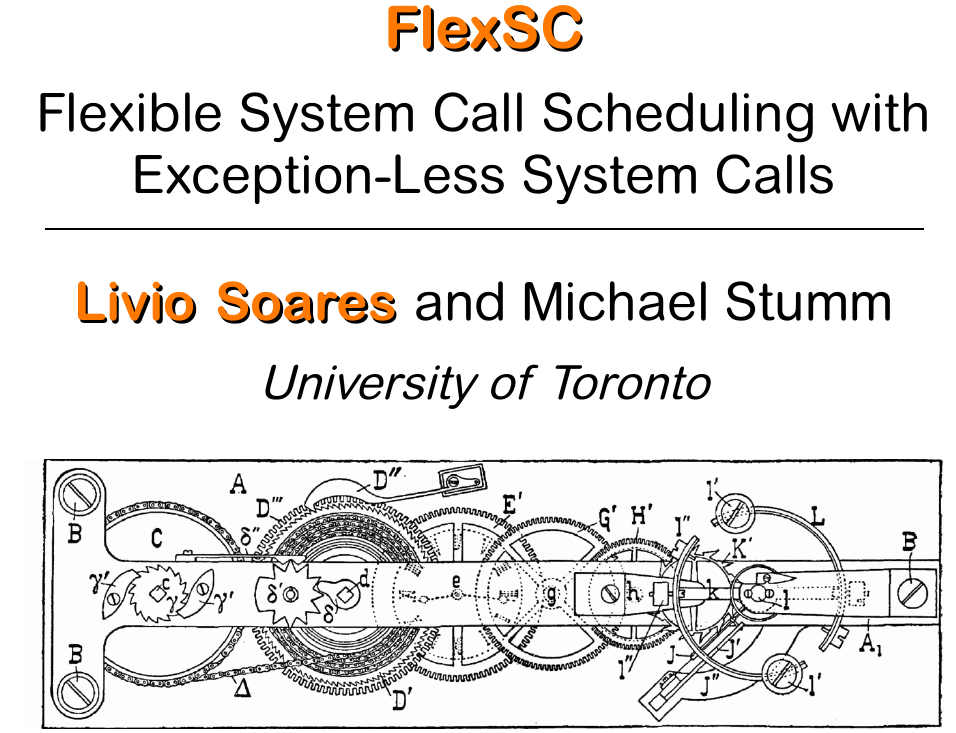
\includegraphics[width=1.\textwidth]{flexsc}


		\end{column}

\begin{column}{.3\textwidth}
	
	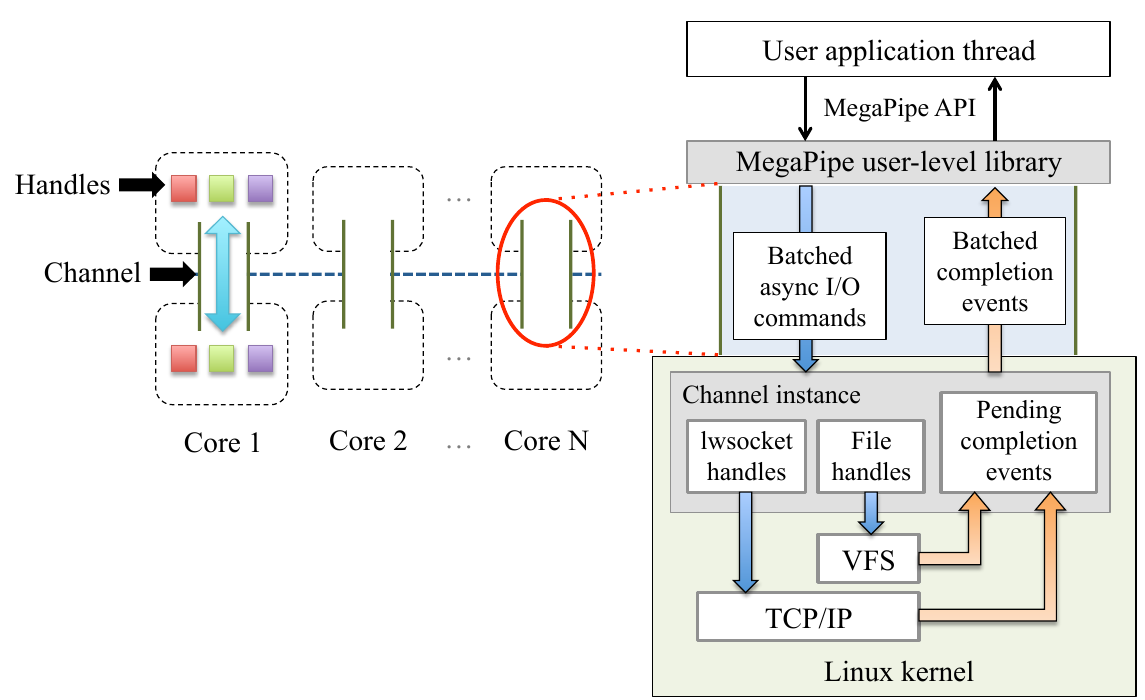
\includegraphics[width=1.\textwidth]{megapipe}
\end{column}



\begin{column}{.3\textwidth}	
		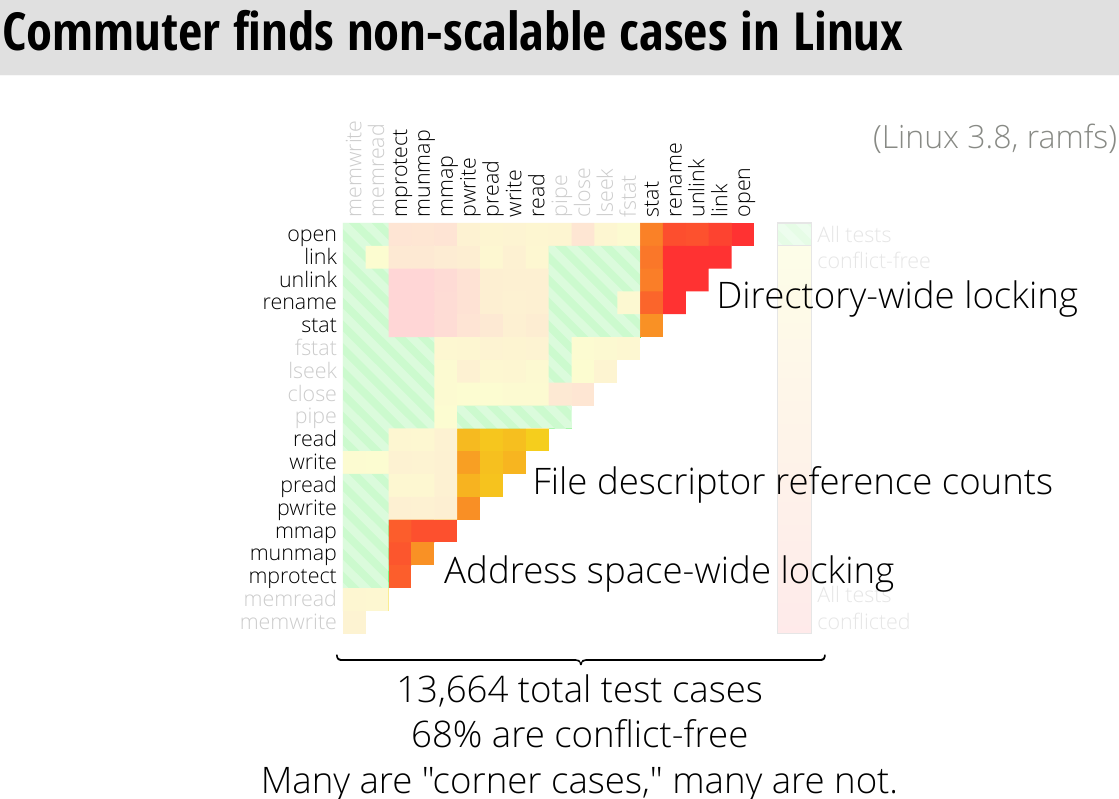
\includegraphics[width=1.\textwidth]{commuter}
\end{column}

\end{columns}

Reference: \\
\tiny Flexsc: Flexible System Call Scheduling with Exception-Less System Calls,OSDI 2010 \\
\tiny MegaPipe: A New Programming Interface for Scalable Network I/O, OSDI 2012 \\
\tiny The Scalable Commutativity Rule: Designing Scalable Software for Multicore Processors, SOSP 2013.  


\end{frame}	


%-------------------------------------------------
\begin{frame}[plain]
	\frametitle{Introduction}
	
	
	\begin{columns}
		
		\begin{column}{.3\textwidth}	
			
			%			\centering
			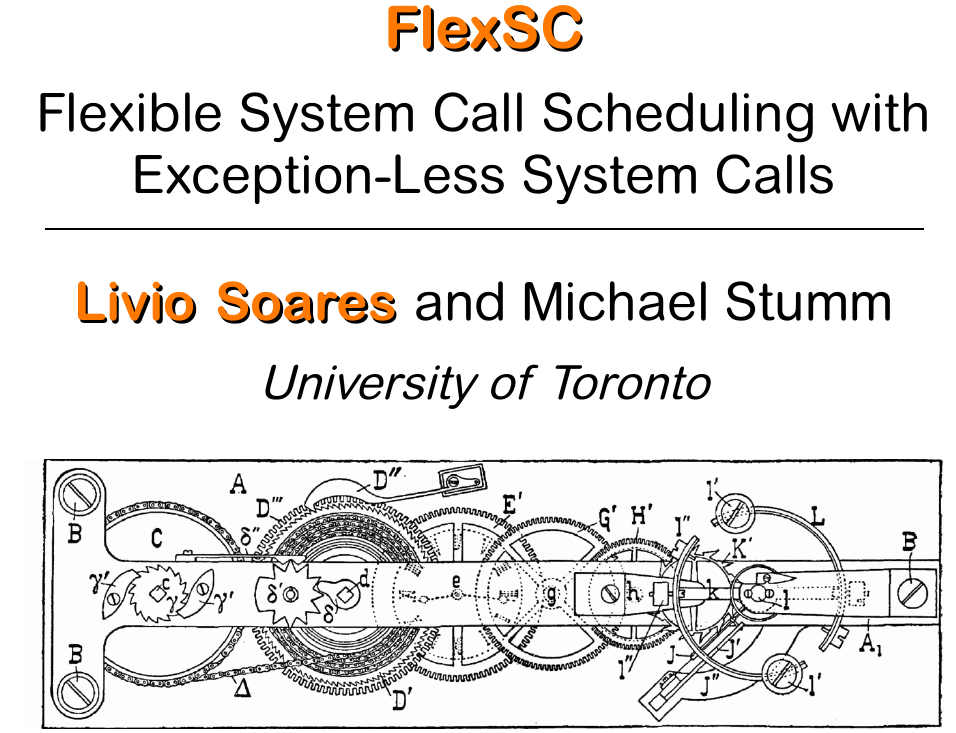
\includegraphics[width=1.\textwidth]{flexsc}
			
			
		\end{column}
		
		\begin{column}{.3\textwidth}
			
			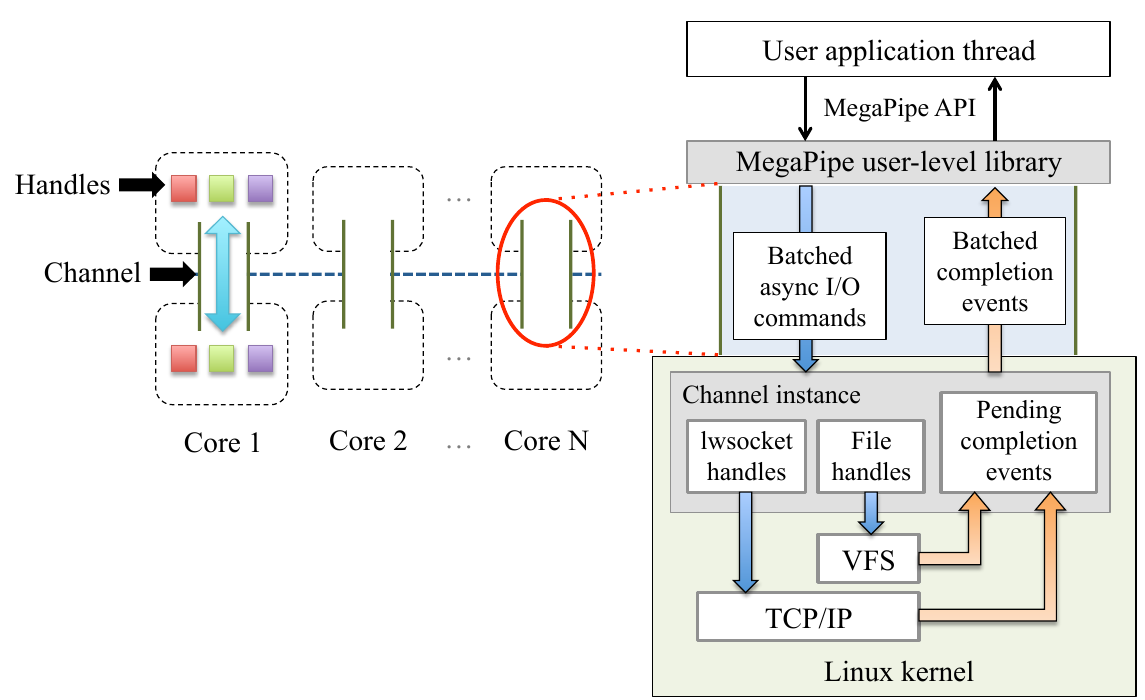
\includegraphics[width=1.\textwidth]{megapipe}
		\end{column}
		
		
		
		\begin{column}{.3\textwidth}	
			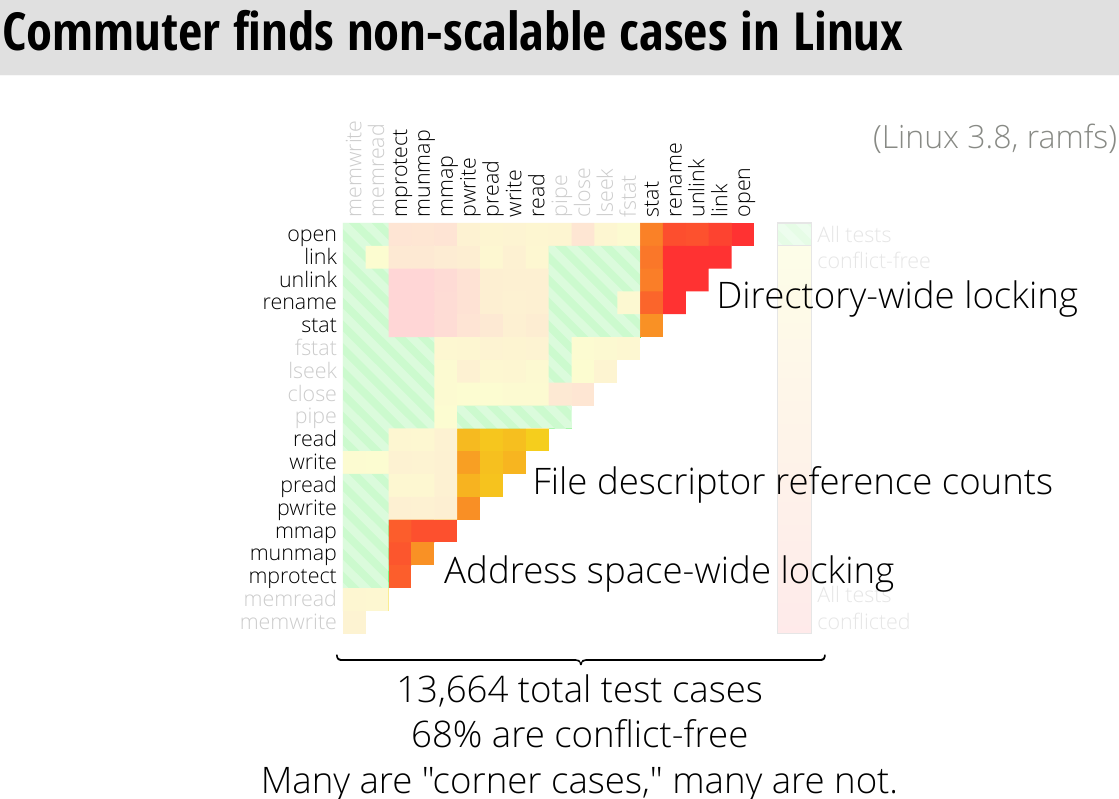
\includegraphics[width=1.\textwidth]{commuter}
		\end{column}
		
	\end{columns}
	
%	\centering
	Improve performance: 
	\begin{itemize}
		\item synchronmous syscall is a legacy
		\item syscall is not for high-speed net
		\item syscall is not for multicore arch
	\end{itemize}
	
	
\end{frame}	

%-------------------------------------------------
\begin{frame}[plain]
	\frametitle{Introduction -- FlexSC}
	
	
	\begin{columns}
		
		\begin{column}{.3\textwidth}	
			
			%			\centering
			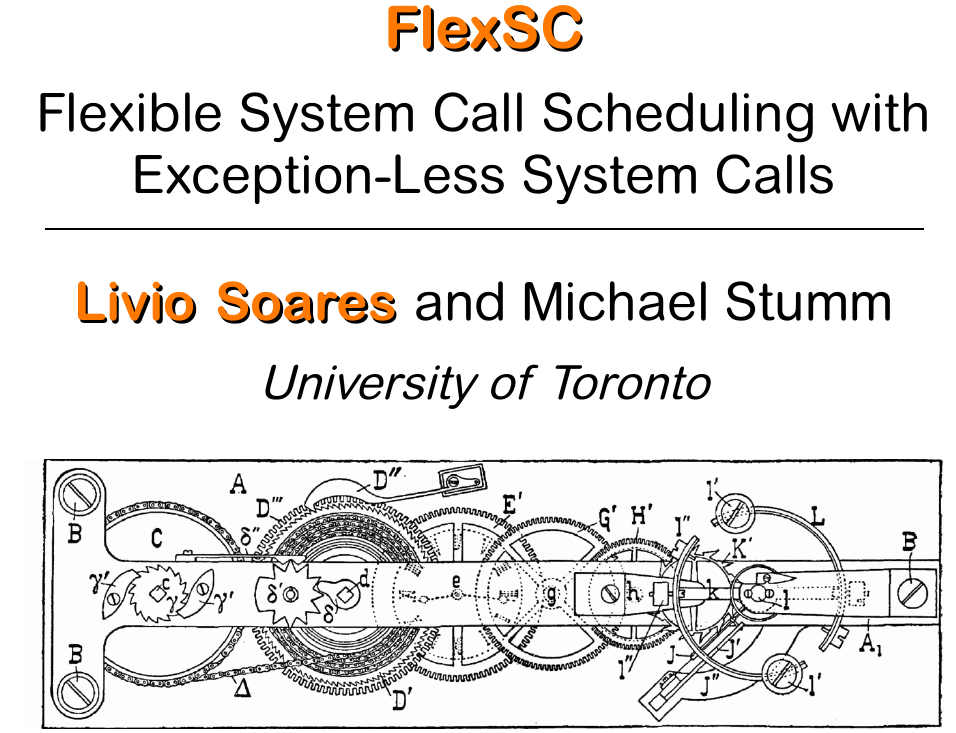
\includegraphics[width=1.\textwidth]{flexsc}
			
			
		\end{column}
		
		\begin{column}{.7\textwidth}
		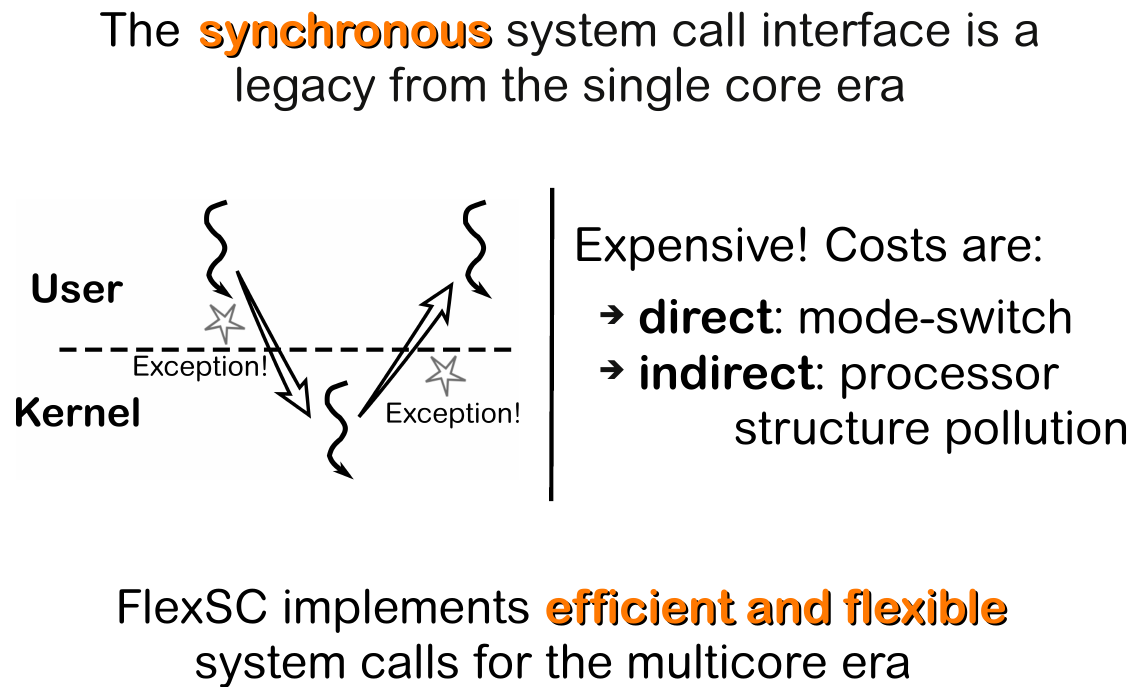
\includegraphics[width=1.\textwidth]{flexsc-motivation}
		\end{column}
		
	\end{columns}
	
	
\end{frame}	


%-------------------------------------------------
\begin{frame}[plain]
	\frametitle{Introduction -- FlexSC}
	
	
	\begin{columns}
		
		\begin{column}{.3\textwidth}	
			
			%			\centering
			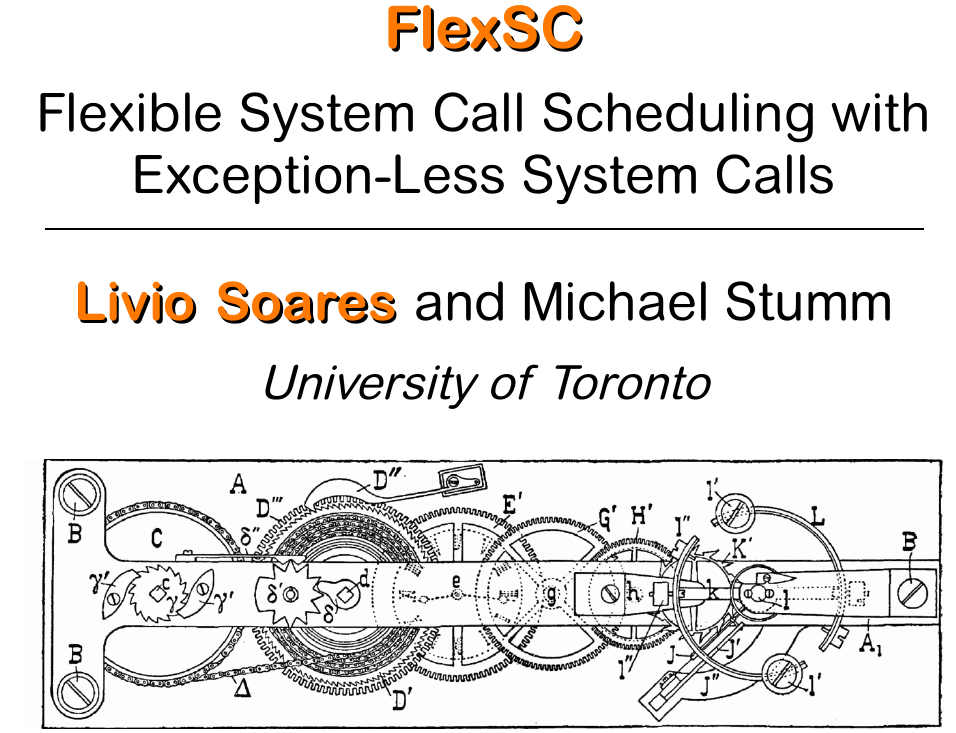
\includegraphics[width=1.\textwidth]{flexsc}
			
			
		\end{column}
		
		\begin{column}{.7\textwidth}
			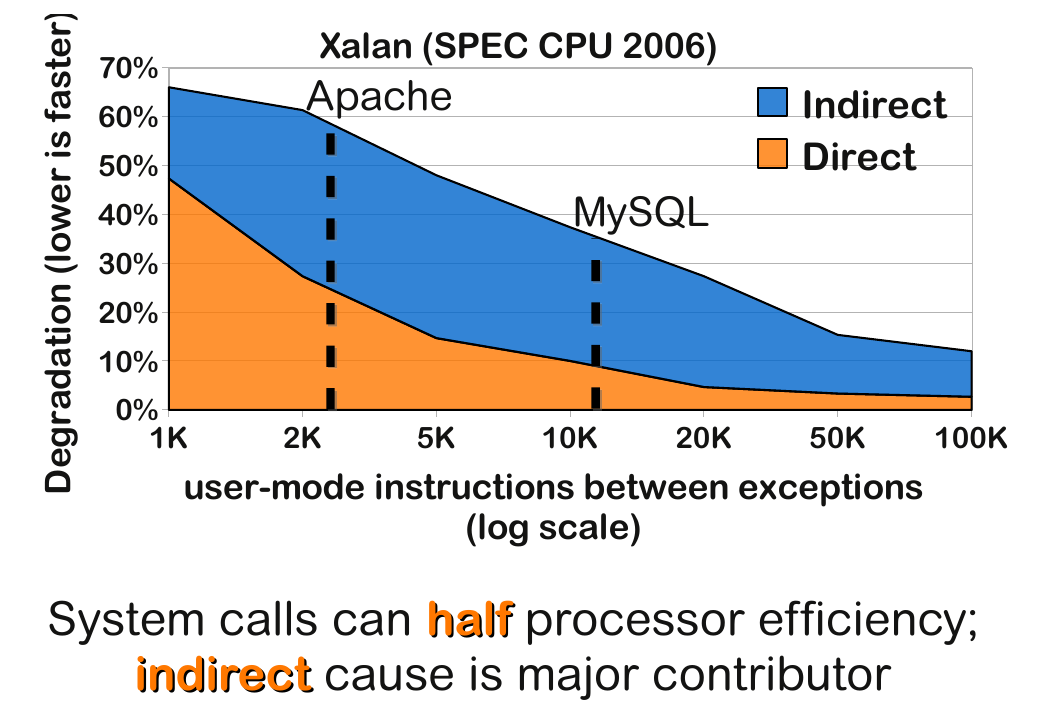
\includegraphics[width=1.\textwidth]{flexsc-slow-sync-syscall}
		\end{column}
		
	\end{columns}
	
	
\end{frame}	



%-------------------------------------------------
\begin{frame}[plain]
	\frametitle{Introduction -- FlexSC}
	
	
	\begin{columns}
		
		\begin{column}{.4\textwidth}	
			
			%			\centering
%			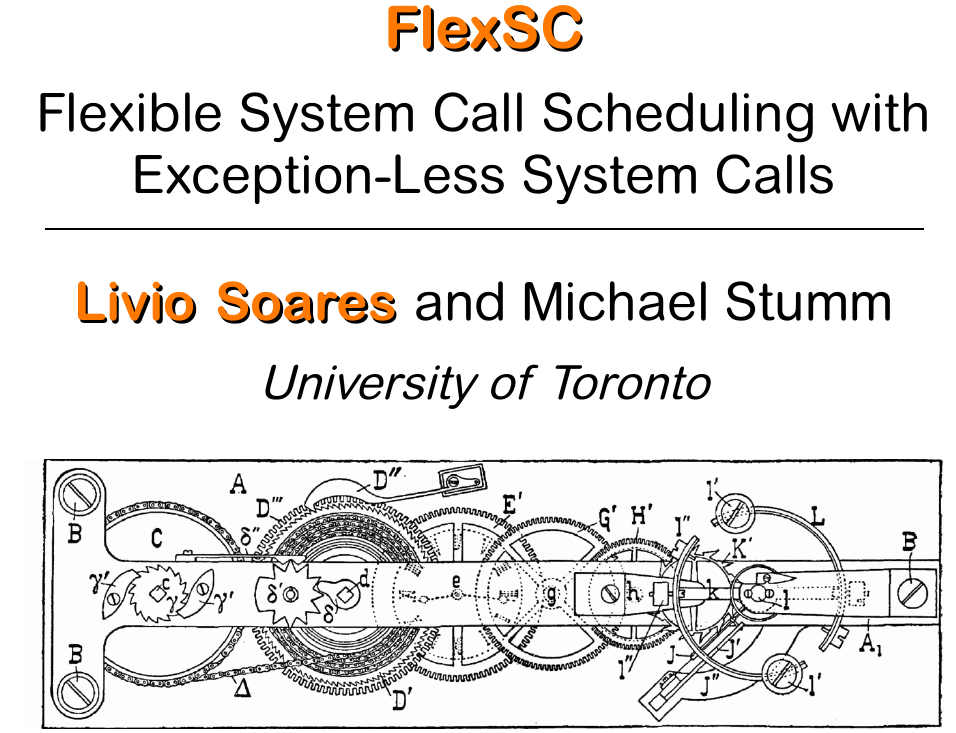
\includegraphics[width=1.\textwidth]{flexsc}
			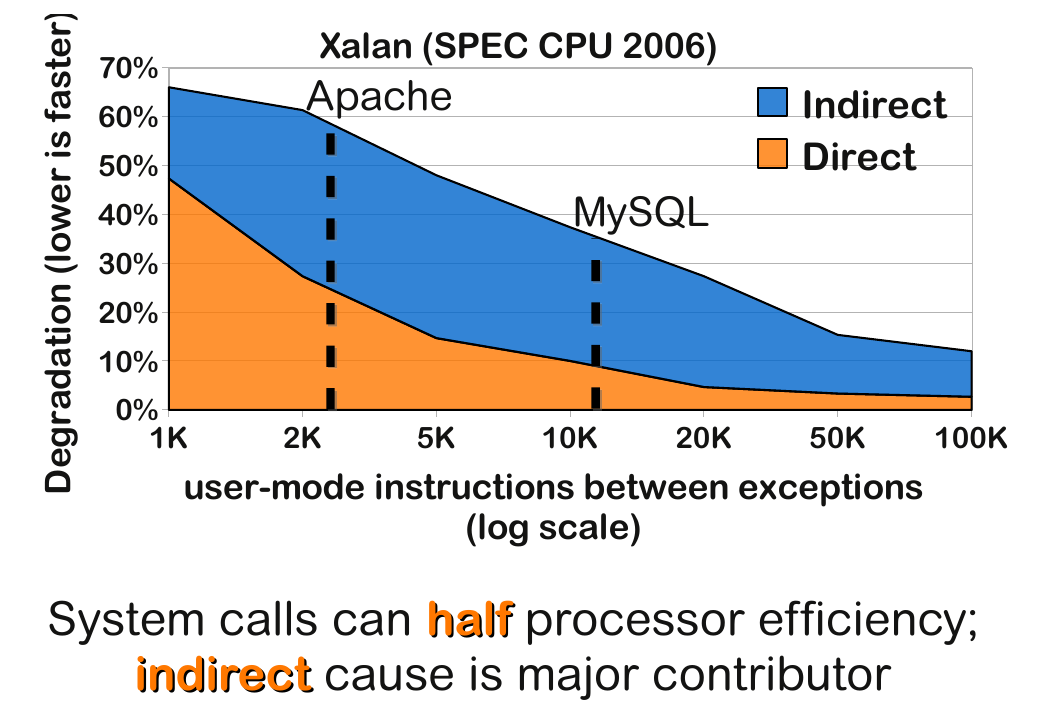
\includegraphics[width=1.\textwidth]{flexsc-slow-sync-syscall}
			
		\end{column}
		
		\begin{column}{.6\textwidth}
			
		Key source of performance impact
		\begin{itemize}
			\item  Traditional system calls are synchronous
			and use exceptions to cross domains
			
			\item Kernel performance equally affected.
Processor efficiency for OS code is also cut
in half			
			\item On a Linux write() call:
			up to 2/3
			of the L1 data cache and data
			TLB are evicted
			

			
		\end{itemize}
	
		\end{column}
		
	\end{columns}
	
	
\end{frame}	



%-------------------------------------------------
\begin{frame}[plain]
	\frametitle{Introduction -- FlexSC}
	
	
	\begin{columns}
		
		\begin{column}{.4\textwidth}	
			
			%			\centering
			%			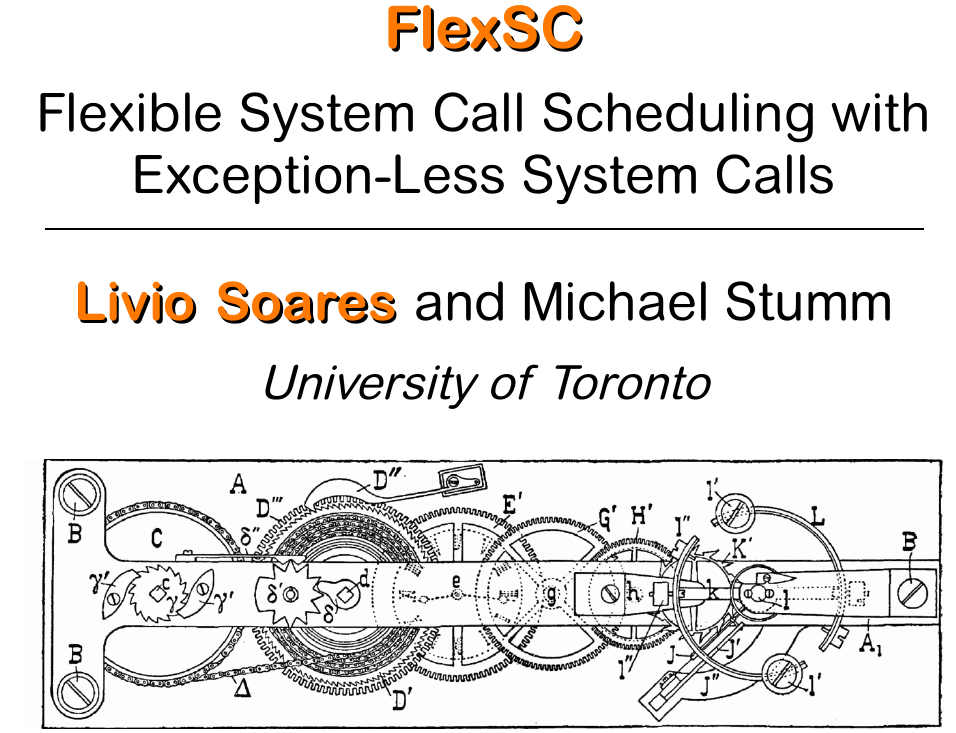
\includegraphics[width=1.\textwidth]{flexsc}
			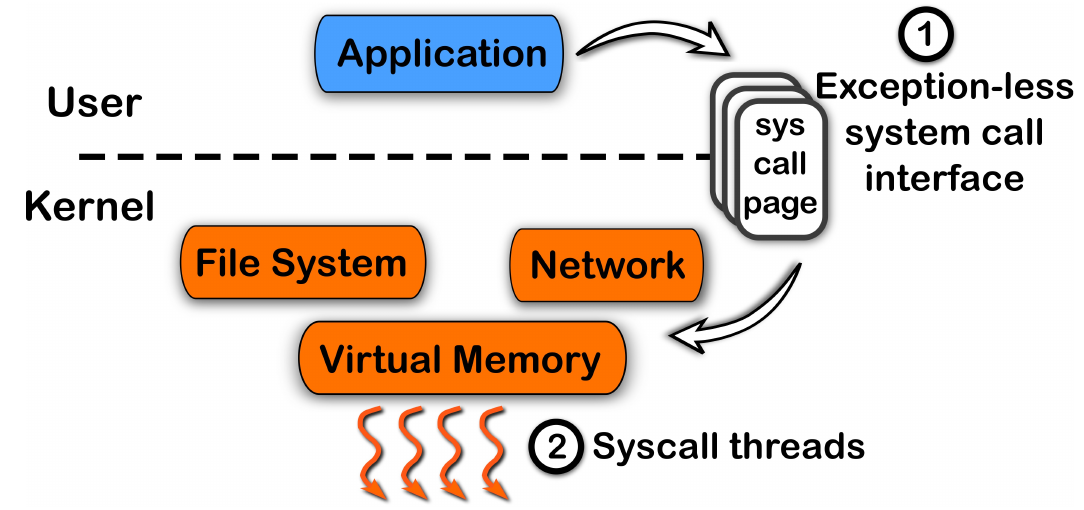
\includegraphics[width=1.\textwidth]{flexsc-arch}
			
		\end{column}
		
		\begin{column}{.6\textwidth}
			
			Exception-less syscalls
			\begin{itemize}
				\item  Remove synchronicity
				by decoupling invocation from execution
				
				
				\item Allow for batching, reduce indirect costs, fewer mode switches
				
				
				
				\item Allow for dynamic multicore specialization
				
				
				
			\end{itemize}
			
		\end{column}
		
	\end{columns}
	
	
\end{frame}	


%-------------------------------------------------
\begin{frame}[plain]
	\frametitle{Introduction -- FlexSC}
	
	
	\begin{columns}
		
		\begin{column}{.4\textwidth}	
			
			%			\centering
			%			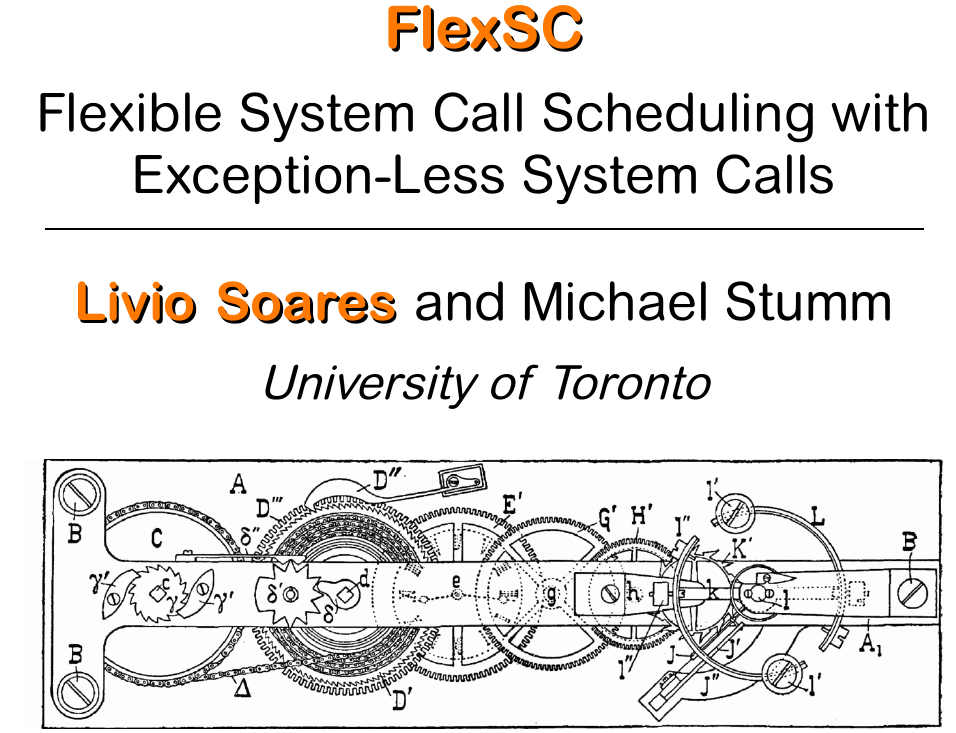
\includegraphics[width=1.\textwidth]{flexsc}
			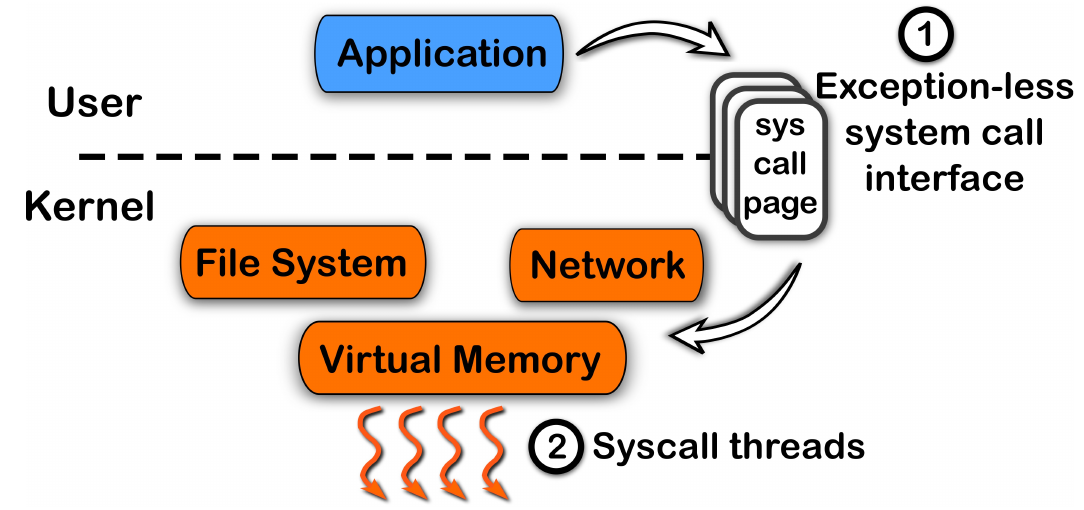
\includegraphics[width=1.\textwidth]{flexsc-arch}
			
		\end{column}
		
		\begin{column}{.6\textwidth}
			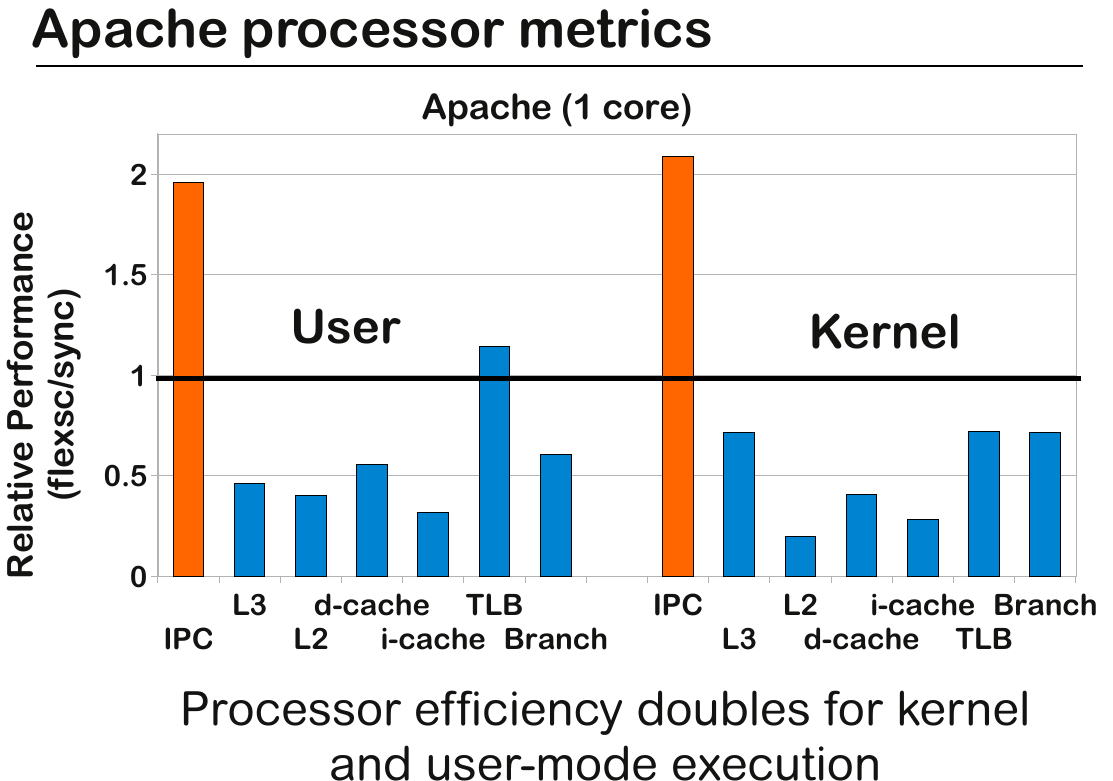
\includegraphics[width=1.\textwidth]{flexsc-perf}


			
		\end{column}
		
	\end{columns}

			\LARGE Contributions: Exception-less syscalls  \& FlexSC-Threads	
	
\end{frame}	
%-------------------------------------------------

%-------------------------------------------------
\end{document}